\chapter{Avaliação Empírica do Sistema de Recomendação}
\label{sec:avaliacao_recomendacao}
Na Literatura é possível encontrar algumas dimensões para avaliação de RSSE, e as recomendações providas por ele. Em \citet{robillard2010recommendation} são apresentadas 16 dimensões de avaliação para um RSSE, que estão apresentadas na \ref{tab:dimensoes}. Cada dimensão possui sua técnica de avaliação, algumas são quantitativas outras qualitativas, algumas possuem as duas abordagens.

\begin{table}[]
	\centering
	\caption{Dimensões de avaliação para RSSE. Tradução de \citet{robillard2010recommendation}}
	\label{tab:dimensoes}
	\begin{tabular}{|l|l|l|ll}
		\cline{1-3}
		\multicolumn{1}{|c|}{\cellcolor[HTML]{C0C0C0}\textbf{Dimensão}} & \multicolumn{1}{c|}{\cellcolor[HTML]{C0C0C0}\textbf{Descrição}} & \multicolumn{1}{c|}{\cellcolor[HTML]{C0C0C0}\textbf{Tipo de métrica}} &  &  \\ \cline{1-3}
		Corretude & \begin{tabular}[c]{@{}l@{}}Quão próximo é a recomendação do \\ conjunto de recomendações que \\ assumimos ser corretas?\end{tabular} & quantitativa &  &  \\ \cline{1-3}
		Cobertura & \begin{tabular}[c]{@{}l@{}}Até que ponto a cobertura do SR sobre \\ um conjunto de itens ou o espaço do usuário?\end{tabular} & quantitativa &  &  \\ \cline{1-3}
		Diversidade & Qual a diversidade das recomendações? & quantitativa &  &  \\ \cline{1-3}
		Confiável & Como a recomendação pode ser confiável? & qualitativa &  &  \\ \cline{1-3}
		Confiança do SR & Quão confiante o SR é? & \begin{tabular}[c]{@{}l@{}}quantitativa / \\ qualitativa\end{tabular} &  &  \\ \cline{1-3}
		Novidade & \begin{tabular}[c]{@{}l@{}}Qual é o sucesso do SR em gerar novas \\ recomendações ou recomendações ainda \\ desconhecidas para o usuário?\end{tabular} & \begin{tabular}[c]{@{}l@{}}quantitativa / \\ qualitativa\end{tabular} &  &  \\ \cline{1-3}
		Acaso & \begin{tabular}[c]{@{}l@{}}Até que ponto o SR ainda promove \\ surpresa com sucesso?\end{tabular} & \begin{tabular}[c]{@{}l@{}}quantitativa /\\ qualitativa\end{tabular} &  &  \\ \cline{1-3}
		Utilidade & \begin{tabular}[c]{@{}l@{}}Qual é o ganho de valor dessa \\ recomendação para o usuário?\end{tabular} & \begin{tabular}[c]{@{}l@{}}quantitativa / \\ qualitativa\end{tabular} &  &  \\ \cline{1-3}
		Risco & \begin{tabular}[c]{@{}l@{}}Qual é o risco para o usuário \\ aceitar essa recomendação?\end{tabular} & qualitativa &  &  \\ \cline{1-3}
		Robustez & \begin{tabular}[c]{@{}l@{}}Qual é a tolerância do SR para um \\ viés ou uma informação falsa?\end{tabular} & quantitativa &  &  \\ \cline{1-3}
		\begin{tabular}[c]{@{}l@{}}Taxa de \\ Aprendizagem\end{tabular} & \begin{tabular}[c]{@{}l@{}}Quão rápido é o SR para adicionar novas \\ informações ou atualizar a lista de recomendação?\end{tabular} & quantitativa &  &  \\ \cline{1-3}
		Usabilidade & \begin{tabular}[c]{@{}l@{}}O qual usável é o SR? Será fácil dos \\ usuários se adequar de uma forma apropriada?\end{tabular} & \begin{tabular}[c]{@{}l@{}}quantitativa / \\ qualitativa\end{tabular} &  &  \\ \cline{1-3}
		Escalabilidade & \begin{tabular}[c]{@{}l@{}}Quão escalável é o SR em relação \\ ao numero de usuários, levando em \\ consideração o tamanho dos dados e \\ a performance dos algoritmos?\end{tabular} & quantitativa &  &  \\ \cline{1-3}
		Estabilidade & Quão consistente é o SR em um período de tempo? & quantitativa &  &  \\ \cline{1-3}
		Privacidade & Existe algum risco a privacidade do usuário? & \begin{tabular}[c]{@{}l@{}}quantitativa / \\ qualitativa\end{tabular} &  &  \\ \cline{1-3}
		\begin{tabular}[c]{@{}l@{}}Preferência do\\ Usuário\end{tabular} & Como o usuário entende o SR? & \begin{tabular}[c]{@{}l@{}}quantitativa / \\ qualitativa\end{tabular} &  &  \\ \cline{1-3}
	\end{tabular}
\end{table}

\begin{table}[]
	\centering
	\caption{Categorização das 16 dimensões. Tradução de \citet{robillard2010recommendation}}
	\label{tab:dimens-catg}
	\begin{tabular}{@{}llll@{}}
		\toprule
		\begin{tabular}[c]{@{}l@{}}Centralizado na \\ Recomendação\end{tabular} & \begin{tabular}[c]{@{}l@{}}Centralizado no \\ Usuário\end{tabular} & \begin{tabular}[c]{@{}l@{}}Centralizado no \\ Sistema\end{tabular} & \begin{tabular}[c]{@{}l@{}}Centralizado na \\ Entrega\end{tabular} \\ \midrule
		Corretude & Confiável & Robustez & Usabilidade \\
		Cobertura & Novidade & Taxa de Aprendizagem & Preferência do usuário \\
		Diversidade & Acaso & Escalabilidade &  \\
		Confiança do SR & Utilidade & Estabilidade &  \\
		& Risco & Privacidade &  \\ \bottomrule
	\end{tabular}
\end{table}

Essas dimensões podem ser subdivididas em categorias como mostra a \ref{tab:dimens-catg}. As dimensões centradas na recomendação avaliam principalmente as recomendações geradas pelo próprio sistema de recomendação. As dimensões centradas no usuário nos permitem avaliar se o sistema de recomendação atende às necessidades do seu usuário final. As dimensões centradas no sistema, em contraste a dimensões anterior, estas fornecem principalmente formas de avaliar o próprio sistema de recomendação ao invés das recomendações. Finalmente, as dimensões centradas na entrega estão focadas principalmente no contexto de uso do sistema de recomendação \cite{robillard2010recommendation}.

\begin{figure}[htb]
	\centering					
	{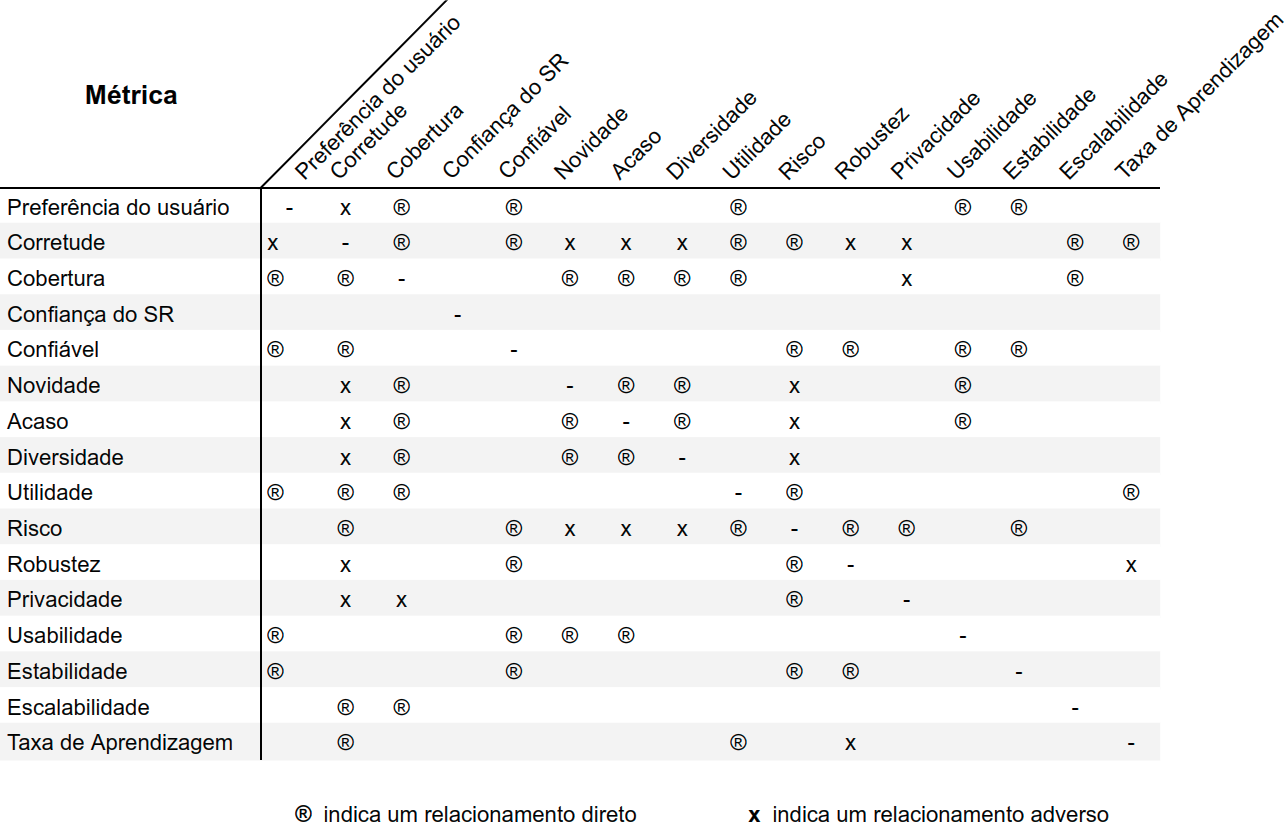
\includegraphics[scale=.4]{rel_metricas_pt.png}}
	
	\caption{Cruzamento de interesses entre as dimensões. Traduzido e adaptado de \citet{robillard2010recommendation}}
	\label{fig:rel_metricas}
\end{figure}

A \ref{fig:rel_metricas} apresenta o relacionamentos direto e adverso entro as métricas de avaliação. Por exemplo, o relacionamento direto entre as métricas Corretude e Cobertura, significa que, se o RSSE possui a métrica Corretude  provavelmente terá a métrica de Cobertura. No caso do relacionamento adverso, por exemplo, as métricas Corretude e Diversidade, significa que, se o RSSE possui a métrica Corretude provavelmente não terá a métrica Diversidade